% +--------------------------------------------------------------------+
% | LaTeX Template for K-State Electronic Theses, Dissertations,
% | and Reports
% |
% | Some guidelines for using the template are shown in comments.  Read
% | these comments carefully, as they describe changes you will need to
% | make to the template in order to meet Graduate School requirements.            |
% |
% | Additional information on using the template are contained in these
% | files, which are included when you download the template:
% |
% | ReadMe.pdf - A general overview of using the template
% |
% | BibTeX Guide.pdf - Detailed guidelines on using BibTeX to create
% | your bibliography and manage your citations.
% |
% | natbib.pdf - Gives detailed information on using the natbib package
% | and formatting citations
% +--------------------------------------------------------------------+

% +--------------------------------------------------------------------+
% | The template is designed to be used with PDFLaTeX. Process this
% | file (etdrtemplate.tex) with PDFLaTeX in order to produce a PDF
% | version of your ETDR.  If you are using BibTex to manage your
% | refrences, you will need to process your file four times:
% | 1. Run PDFLaTeX
% | 2. Run BibTex
% | 3. Run PDFLaTeX
% | 4. Run PDFLaTeX
% |
% | Some LaTeX editors do not explicitly list PDFLaTeX as an option, but
% | do use PDFLaTeX to produce a PDF file directly from your .tex files.
% | See the ReadMe file for details.
% +--------------------------------------------------------------------+
% |
% +--------------------------------------------------------------------+
% |
% | As required by the Graduate School, The template is configured to
% | contain the following sections in the order shown.

% | Abstract title page (doctoral dissertations only)
% | Abstract (doctoral dissertations only)
% | Title page
% | Copyright page
% | Abstract
% | Table of contents
% | List of figures
% | List of tables
% | Acknowledgements (Optional)
% | Dedication (Optional)
% | Preface (Optional)
% | Individual Chapters
% | References or Bibliography
% | Appendices (as needed)
% |
% | Details on removing optional sections are given in the comments below.
% |
% +--------------------------------------------------------------------+

% +--------------------------------------------------------------------+
% | The LaTex command \documentclass selects a particular class to
% | associate with the document.  Within this command, 12pt is
% | specified for the font size.  You can change this to 11 pt, if
% | desired.
% +--------------------------------------------------------------------+

\documentclass[final,letterpaper,12pt,oneside]{class_diss}

% +--------------------------------------------------------------------+
% | Here are added external packages that will be used throughout
% | the document.  You can add other packages as needed.
% +--------------------------------------------------------------------+

\usepackage{graphicx} % Extended graphics package.
\usepackage{amsmath} % American Mathematics Society standards
\usepackage{amsxtra} % Additional math symbols
\usepackage{amssymb} % Additional math symbols
\usepackage{amsthm} % Additional math symbols
\usepackage{latexsym} % Additional math symbols
\usepackage{setspace} % Controls line spacing
\usepackage[margin=1in]{geometry} % Sets page margins to 1 inch on all sides
\usepackage[titles]{tocloft} % Adds leader dots to all entries in the table of contents

% +--------------------------------------------------------------------+
% |
% | Citation and Bibliography Style
% |
% | The following commands determine the citation and bibliography style.  The
% | template uses BibTeX for formatting the bibliography.  See "BibTeX Guide.pdf"
% | for details on formatting citations and references.  The template is set
% | to use a generic, superscript style, but it can be easily modified
% | to use author-year styles.

\bibliographystyle{unsrtnat}
% | If you want to use an author-year citation style, change "unsrtnat" to
% | "plainnat" in the line above.  You can also use other styles supported
% | by LaTeX, e.g., acm, ieeetr, siam, etc.  Additional styles
% | are in the \styles folder and can be invoked like this:
% | \bibliographystyle{styles/apsrev}.  If the style you use is based
% | on an author-year citation style, you will need to make changes
% | in the usepackage and \setcitestyle statements below

\usepackage[super,sort&compress]{natbib}
% | If you want to use an author-year citation style, change "super" to
% | "authoryear" in the line above.

\setcitestyle{super}
% | if you want to use an author-year citation style, change "super" to
% | "authoryear" in the line above.

% +---------------------------------------------------------------------+
% | The hyperref package enables cross-references.
% +---------------------------------------------------------------------+

\usepackage[pdftex, plainpages=false, pdfpagelabels]{hyperref}

\hypersetup{
    linktocpage=true,
    colorlinks=true,
    bookmarks=true,
    citecolor=blue,
    urlcolor=blue,
    linkcolor=blue,
    citebordercolor={1 0 0},
    urlbordercolor={1 0 0},
    linkbordercolor={.7 .8 .8},
    breaklinks=true,
    pdfpagelabels=true,
    }

% +--------------------------------------------------------------------+
% | The document begins here.
% +--------------------------------------------------------------------+

\doublespacing
\begin{document}

% +--------------------------------------------------------------------+
% | ******Masters Students -- You Need to Make Some Changes Here******
% |
% | The Abstract Title page and Abstract page following the Abstract
% | Title page are required only for doctoral dissertations.  For
% | masters theses or reports, comment out or delete the lines:
% |
% | % +--------------------------------------------------------------------+
% | Abstract Title Page
% |
% |This page is required only for doctoral dissertations.
% +--------------------------------------------------------------------+

% +--------------------------------------------------------------------+
% | This page should not contain a page number.  We use the
% | \thispagestyle[empty] command below to suppress page numbers
% | and other style elements.
% +--------------------------------------------------------------------+

\thispagestyle{empty}

% +--------------------------------------------------------------------+
% | The Abstract Title page begins here
% +--------------------------------------------------------------------+

\pdfbookmark[0]{Title Page}{PDFTitlePage}
%\setcounter{page}{1}

\begin{center}

   \vspace{1cm}

% +--------------------------------------------------------------------+
% | Enter the title of your ETDR below.  Use ALL CAPITAL LETTERS.
% +--------------------------------------------------------------------+

   \large ENTER YOUR TITLE\\

   \vspace{0.5cm}

   by\\

   \vspace{0.5cm}

% +--------------------------------------------------------------------+
% | Enter your name below in ALL CAPITAL LETTERS.
% +--------------------------------------------------------------------+

   \large ENTER YOUR NAME\\

   \vspace{0.5cm}

% +--------------------------------------------------------------------+
% | On the line below, replace "Enter Your Previous Degrees"
% | with your previous degrees in mixed case. Include the abbreviation
% | for the degree, the name of the university, and the year separated
% | by commas. For example:
% |
% |    B.A., University of Illinois, 2000
% |
% | If desired, it is acceptable to include a city or country with
% | the university name. For example:
% |
% |    B.S., Jillian University, China, 2002
% |
% | Each degree should appear on a separate line.  Use the \\
% | command to create a line break.
% +--------------------------------------------------------------------+

   Enter Your Previous Degrees\\

   \vspace{0.55cm}
   \rule{2in}{0.5pt}\\
   \vspace{0.75cm}

   {\large AN ABSTRACT OF A DISSERTATION}\\

   \vspace{0.5cm}
   \begin{singlespace}
   submitted in partial fulfillment of the\\
   requirements for the degree\\
   \end{singlespace}

   \vspace{0.5cm}

% +--------------------------------------------------------------------+
% | On the line below, enter the name of your earned degree in ALL
% | CAPITAL LETTERS.  For example: DOCTOR OF PHILOSOPHY
% +--------------------------------------------------------------------+


   {\large ENTER YOUR DEGREE NAME}\\
   \vspace{0.5cm}

% +--------------------------------------------------------------------+
% | On the two lines below, enter the name of your department and the
% | name of the college in mixed case.  For example:
% |
% |     Biochemistry Department
% |     College of Arts and Sciences
% +--------------------------------------------------------------------+

   \begin{singlespace}
   Enter Your Department Name\\
   Enter Your College Name\\
   \end{singlespace}

   \vspace{0.5cm}

   \begin{singlespace}
   {\Large KANSAS STATE UNIVERSITY}\\
   Manhattan, Kansas\\
   \end{singlespace}

% +--------------------------------------------------------------------+
% | On the line below, replace "Graduation Year" with the four-digit year
% | of your graduation. For example:
% |
% |     2016
% +--------------------------------------------------------------------+

   Graduation Year\\
   \vspace{1cm}

\end{center}
 through \end{abstract}.
% |
% | You will also need to uncomment the two lines following the
% | \begin{abstract} command:
% |    %\setcounter{page}{-1}
% |    %\pdfbookmark[0]{Abstract}{PDFAbstractPage}
% |
% | Don't uncomment the lines above.  Scroll down several lines until
% | you see the section "For masters theses or reports, uncomment
% | the commands..." and uncomment the lines in that section.
% +--------------------- ----------------------------------------------+

% +--------------------------------------------------------------------+
% | Abstract Title Page
% |
% |This page is required only for doctoral dissertations.
% +--------------------------------------------------------------------+

% +--------------------------------------------------------------------+
% | This page should not contain a page number.  We use the
% | \thispagestyle[empty] command below to suppress page numbers
% | and other style elements.
% +--------------------------------------------------------------------+

\thispagestyle{empty}

% +--------------------------------------------------------------------+
% | The Abstract Title page begins here
% +--------------------------------------------------------------------+

\pdfbookmark[0]{Title Page}{PDFTitlePage}
%\setcounter{page}{1}

\begin{center}

   \vspace{1cm}

% +--------------------------------------------------------------------+
% | Enter the title of your ETDR below.  Use ALL CAPITAL LETTERS.
% +--------------------------------------------------------------------+

   \large ENTER YOUR TITLE\\

   \vspace{0.5cm}

   by\\

   \vspace{0.5cm}

% +--------------------------------------------------------------------+
% | Enter your name below in ALL CAPITAL LETTERS.
% +--------------------------------------------------------------------+

   \large ENTER YOUR NAME\\

   \vspace{0.5cm}

% +--------------------------------------------------------------------+
% | On the line below, replace "Enter Your Previous Degrees"
% | with your previous degrees in mixed case. Include the abbreviation
% | for the degree, the name of the university, and the year separated
% | by commas. For example:
% |
% |    B.A., University of Illinois, 2000
% |
% | If desired, it is acceptable to include a city or country with
% | the university name. For example:
% |
% |    B.S., Jillian University, China, 2002
% |
% | Each degree should appear on a separate line.  Use the \\
% | command to create a line break.
% +--------------------------------------------------------------------+

   Enter Your Previous Degrees\\

   \vspace{0.55cm}
   \rule{2in}{0.5pt}\\
   \vspace{0.75cm}

   {\large AN ABSTRACT OF A DISSERTATION}\\

   \vspace{0.5cm}
   \begin{singlespace}
   submitted in partial fulfillment of the\\
   requirements for the degree\\
   \end{singlespace}

   \vspace{0.5cm}

% +--------------------------------------------------------------------+
% | On the line below, enter the name of your earned degree in ALL
% | CAPITAL LETTERS.  For example: DOCTOR OF PHILOSOPHY
% +--------------------------------------------------------------------+


   {\large ENTER YOUR DEGREE NAME}\\
   \vspace{0.5cm}

% +--------------------------------------------------------------------+
% | On the two lines below, enter the name of your department and the
% | name of the college in mixed case.  For example:
% |
% |     Biochemistry Department
% |     College of Arts and Sciences
% +--------------------------------------------------------------------+

   \begin{singlespace}
   Enter Your Department Name\\
   Enter Your College Name\\
   \end{singlespace}

   \vspace{0.5cm}

   \begin{singlespace}
   {\Large KANSAS STATE UNIVERSITY}\\
   Manhattan, Kansas\\
   \end{singlespace}

% +--------------------------------------------------------------------+
% | On the line below, replace "Graduation Year" with the four-digit year
% | of your graduation. For example:
% |
% |     2016
% +--------------------------------------------------------------------+

   Graduation Year\\
   \vspace{1cm}

\end{center}
  % Masters students - comment or delete this line

\begin{abstract} % Masters students - comment or delete this line
   \setcounter{page}{-1} % Masters students - comment or delete this line
   \pdfbookmark[0]{Abstract}{PDFAbstractPage} % Masters students - comment or delete this line
   % +--------------------------------------------------------------------+
% | Abstract Page
% +--------------------------------------------------------------------+

\pagestyle{empty}
%\vspace{1cm}
\setlength{\baselineskip}{0.8cm}

%\indent

% +--------------------------------------------------------------------+
% | Enter the text of your abstract below, maximum of 500 words.
% +--------------------------------------------------------------------+

Enter the text of your abstract in the abstract.tex file.  Be sure
to delete the text below before you submit your ETDR.

This template uses a separate file for each section of your ETDR:
title page, abstract, preface, chapters, reference, etc.  This
makes it easier to organize and work with a lengthy document.  The
template is configured with page margins required by the Graduate
School and will automatically create a table of contents, lists of
tables and figures, and PDF bookmarks.

The file etdrtemplate.tex is the "master" file for the ETDR
template.  This is the file you need to process with PDFLaTeX in
order to produce a PDF version of your ETDR.  See the comments in
the etdrtemplate.tex and other files for details on using the
template.  You are not required to use the template, but it can save
time and effort in making sure your ETDR meets the Graduate School
formatting requirements.

Although the template gives you a foundation for creating your
ETDR, you will need a working knowledge of LaTeX in order to
produce a final document.  You should be familiar with LaTeX
commands for formatting text, equations, tables, and other
elements you will need to include in your ETDR.
 % Masters students - comment or delete this line
   \vfill % Masters students - comment or delete this line
\end{abstract} % Masters students - comment or delete this line

% +--------------------------------------------------------------------+
% | Title Page -- Required for both Doctoral and Masters Students
% +--------------------------------------------------------------------+

% +--------------------------------------------------------------------+
% | Title Page
% +--------------------------------------------------------------------+

\newpage

% +--------------------------------------------------------------------+
% | This page should not contain a page number.  We use the
% | \thispagestyle[empty] command below to suppress page numbers
% | and other style elements.
% +--------------------------------------------------------------------+

\thispagestyle{empty}

% +--------------------------------------------------------------------+
% | The Title page begins here.
% +--------------------------------------------------------------------+

\begin{center}

   \vspace{1cm}

% +--------------------------------------------------------------------+
% | On the line below, replace "ENTER YOUR TITLE" with the title of
% | your ETDR.  Use all CAPITAL LETTERS.
% +--------------------------------------------------------------------+

   \large ENTER YOUR TITLE\\

   \vspace{0.3cm}

   by\\

   \vspace{0.3cm}

% +--------------------------------------------------------------------+
% | On the line below, replace "ENTER YOUR NAME" with your name.  Use
% | mixed case, for example, Laura Bush.
% +--------------------------------------------------------------------+

   \large Maria I. Pinilla\\

   \vspace{0.3cm}

% +--------------------------------------------------------------------+
% | On the line below, replace "Enter Your Previous Degrees"
% | with your previous degrees in mixed case. Include the abbreviation
% | for the degree, the name of the university, and the year separated
% | by commas. For example:
% |
% |    B.A., University of Illinois, 2000
% |
% | If desired, it is acceptable to include a city or country with
% | the university name. For example:
% |
% |    B.S., Jillian University, China, 2002
% |
% | Each degree should appear on a separate line.  Use the \\
% | command to create a line break.
% +--------------------------------------------------------------------+

   B.S., Kansas State University, 2014\\

   \vspace{0.35cm}
   \rule{2in}{0.5pt}\\
   \vspace{0.65cm}

   {\large A THESIS}\\

   \vspace{0.3cm}
   \begin{singlespace}
   submitted in partial fulfillment of the\\
   requirements for the degree\\
   \end{singlespace}

   \vspace{0.3cm}

% +--------------------------------------------------------------------+
% | On the line below, replace "ENTER YOUR DEGREE NAME" with the name
% | of your earned degree in ALL CAPITAL LETTERS.
% +--------------------------------------------------------------------+

   {\large M.S. NUCLEAR ENGINEERING}\\
   \vspace{0.3cm}

% +--------------------------------------------------------------------+
% | On the two lines below, replace "Enter Your Department Name" and
% | "Enter Your College Name" with the name of your department and the
% | name of the college in mixed case.  For example:
% |
% |     Biochemistry Department
% |     College of Arts and Sciences
% +--------------------------------------------------------------------+

   \begin{singlespace}
   Mechanical and Nuclear Engineering Department\\
   College of Engineering\\
   \end{singlespace}

   \vspace{0.3cm}

   \begin{singlespace}
   {\large KANSAS STATE UNIVERSITY}\\
   Manhattan, Kansas\\
   \end{singlespace}

% +--------------------------------------------------------------------+
% | On the line below, replace "Graduation Year" with the four-digit
% | year of your graduation.  For example:
% |
% |     2016
% +--------------------------------------------------------------------+

   2016\\
   \vspace{0.3cm}

    \end{center}

    \begin{flushright}
    Approved by:\\
    \vspace{0.3cm}
    \begin{singlespace}
    Major Professor


% +--------------------------------------------------------------------+
% | On the line below, replace "Enter Your Major Professor's Name"
% | with  the name of your major professor in mixed case.  Use the
% | format Firstname Lastname.  For example:
% |
% |     Lori Goetsch
% |
% +--------------------------------------------------------------------+

    Dr. William L. Dunn\\
    \end{singlespace}
    \end{flushright}

% +--------------------------------------------------------------------+
% | If you have co-major professors, comment out the lines above from
% | \begin{flushright} through \end{flushright} and uncomment the
% | lines below.  Enter your co-major professors' names where indicated.
% +--------------------------------------------------------------------+

%\begin{flushright}
%   Approved by:\\
%  \vspace{ 0.3cm}
%   \begin{singlespace}
%   Co-Major Professor\\
%   Enter Your Co-Major Professor's Name\\
%   \vspace{.25cm}
%   Co-Major Professor\\
%   Enter Your Co-Major Professor's Name\\
%   \end{singlespace}
%\end{flushright}


% +--------------------------------------------------------------------+
% | Copyright Page -- Required for both Doctoral and Masters Students
% +--------------------------------------------------------------------+

% +--------------------------------------------------------------------+
% | Copyright Page
% +--------------------------------------------------------------------+

\newpage

\thispagestyle{empty}

\vspace*{0.9cm}

\begin{center}

{\bf \Huge Copyright}

\vspace{1cm}

% +--------------------------------------------------------------------+
% | On the line below, replace "Enter Your Name" with your name
% | Use the same form of your name as it appears on your title page.
% | Use mixed case, for example, Barack Obama.
% +--------------------------------------------------------------------+

   \Large Maria I. Pinilla\\

   \vspace{0.5cm}

% +--------------------------------------------------------------------+
% | On the line below, replace "Graduation Year" with the four-digit year
% | of your graduation. For example:
% |
% |     2016
% |
% +--------------------------------------------------------------------+

   2016\\

   \vspace{0.5cm}

\end{center}


% +--------------------------------------------------------------------+
% |  Abstract -- Required for both Doctoral and Masters Students
% +--------------------------------------------------------------------+

\begin{abstract}

% +--------------------------------------------------------------------+
% | For masters theses or reports, uncomment the commands on the next
% | two lines (\setcounter and \pdfbookmark)
% +--------------------------------------------------------------------+

   %\setcounter{page}{-1}
   %\pdfbookmark[0]{Abstract}{PDFAbstractPage}

% +--------------------------------------------------------------------+
% | Abstract Page
% +--------------------------------------------------------------------+

\pagestyle{empty}
%\vspace{1cm}
\setlength{\baselineskip}{0.8cm}

%\indent

% +--------------------------------------------------------------------+
% | Enter the text of your abstract below, maximum of 500 words.
% +--------------------------------------------------------------------+

Enter the text of your abstract in the abstract.tex file.  Be sure
to delete the text below before you submit your ETDR.

This template uses a separate file for each section of your ETDR:
title page, abstract, preface, chapters, reference, etc.  This
makes it easier to organize and work with a lengthy document.  The
template is configured with page margins required by the Graduate
School and will automatically create a table of contents, lists of
tables and figures, and PDF bookmarks.

The file etdrtemplate.tex is the "master" file for the ETDR
template.  This is the file you need to process with PDFLaTeX in
order to produce a PDF version of your ETDR.  See the comments in
the etdrtemplate.tex and other files for details on using the
template.  You are not required to use the template, but it can save
time and effort in making sure your ETDR meets the Graduate School
formatting requirements.

Although the template gives you a foundation for creating your
ETDR, you will need a working knowledge of LaTeX in order to
produce a final document.  You should be familiar with LaTeX
commands for formatting text, equations, tables, and other
elements you will need to include in your ETDR.

\vfill
\end{abstract}

% +--------------------------------------------------------------------+
% | The following commands start a new page and set the page numbering
% | to lowercase roman numerals.
% +--------------------------------------------------------------------+

\newpage
\pagenumbering{roman}

% +--------------------------------------------------------------------+
% |
% | *********************** IMPORTANT ******************************
% |
% | In the \setcounter command below, set the number to represent the
% | page number of the table of contents page.  For example, if the
% | table of contents page is the 6th page of your document, enter 6
% | in the brackets.  This number may vary, depending on the length of
% | your abstract.
% |
% | Numbers do not appear on the title and abstract pages, but they
% | are included in the page count.  The table of contents page is the
% | first page on which page numbers are displayed.
% +--------------------------------------------------------------------+

\setcounter{page}{6}

% +--------------------------------------------------------------------+
% | The following command creates a bookmark for the table of contents
% | in the final PDF document.
% +--------------------------------------------------------------------+

\pdfbookmark[0]{\contentsname}{contents}

% +--------------------------------------------------------=-----------+
% | The following command adds dot leaders for all entries in the
% | table of contents.
% +--------------------------------------------------------------------+

\renewcommand{\cftchapleader}{\cftdotfill{\cftdotsep}}

% +--------------------------------------------------------------------+
% | The following commands makes all entries and page numbers in the
% | table of contents appear in normal weight font (not bold).
% +--------------------------------------------------------------------+

\renewcommand{\cftchapfont}{\mdseries}
\renewcommand{\cftchappagefont}{\mdseries}

% +--------------------------------------------------------------------+
% | These commands add the table of contents, list of figures, and
% | list of tables.
% +--------------------------------------------------------------------+

\tableofcontents
\listoffigures
\listoftables

% +--------------------------------------------------------------------+
% | Acknowledgements Page
% |
% | If you choose not to have an Acknowledgements page, comment out
% | or delete the following 3 lines.
% +--------------------------------------------------------------------+

\phantomsection
\addcontentsline{toc}{chapter}{Acknowledgements}
% +--------------------------------------------------------------------+
% | Acknowledgements Page (Optional)
% +--------------------------------------------------------------------+

\newpage
\vspace*{0.9cm}
\begin{center}
{\bf \Huge Acknowledgments}
\end{center}

\setlength{\baselineskip}{0.8cm}

%\pdfbookmark[0]{Acknowledgements}{PDF_Acknowledgements}

% +--------------------------------------------------------------------+
% | Enter text for your acknowledgements in the space below this box.
% |                                                                    
% +--------------------------------------------------------------------+

Enter the text for your Acknowledgements page in the acknowledge.tex
file. The Acknowledgements page is optional.  If you wish to remove
it, see the comments in the etdrtemplate.tex file.


% +--------------------------------------------------------------------+
% | Dedication Page
% |
% | If you choose not to have a Dedication page, comment out
% | or delete the following 3 lines.
% +--------------------------------------------------------------------+

\phantomsection
\addcontentsline{toc}{chapter}{Dedication}
% +--------------------------------------------------------------------+
% | Dedication Page (Optional)
% +--------------------------------------------------------------------+

\newpage
\vspace*{0.9cm}
\begin{center}
{\bf \Huge Dedication}
\end{center}

\setlength{\baselineskip}{0.8cm}

%\pdfbookmark[0]{Dedication}{PDF_Dedication}

% +--------------------------------------------------------------------+
% | Enter the text for your dedication in the space below this box.    
% +--------------------------------------------------------------------+

Thanks everyone. 


% +--------------------------------------------------------------------+
% | Preface Page
% |
% | If you choose not to have a Dedication page, comment out
% | or delete the following 3 lines.
% +--------------------------------------------------------------------+

\phantomsection
\addcontentsline{toc}{chapter}{Preface}
% +--------------------------------------------------------------------+
% | Preface (Optional)
% +--------------------------------------------------------------------+

\newpage
\vspace*{0.9cm}
\begin{center}
{\bf \Huge Preface}
\end{center}

\setlength{\baselineskip}{0.8cm}

%\pdfbookmark[0]{Preface}{PDF_Preface}

% +--------------------------------------------------------------------+
% | Enter text of your Preface in the space below this box.            
% +--------------------------------------------------------------------+

Enter the text for your Preface page in the preface.tex file. The
Preface page is optional.  If you wish to remove it, see the
comments in the etdrtemplate.tex file.



% +--------------------------------------------------------------------+
% | This is where the chapter content of your ETDR begins.
% +--------------------------------------------------------------------+

%\phantomsection
\newpage
\pagenumbering{arabic}
\setcounter{page}{1}

% +--------------------------------------------------------------------+
% | Individual chapters of your ETDR are added using the \input
% | command.
% +--------------------------------------------------------------------+

% +--------------------------------------------------------------------+
% | Sample Chapter 1
% |
% | This file provides examples of how to
% | - insert a figure with a caption
% | - construct a table with a caption
% | - create subsections within the chapter
% | - insert a reference to a Figure or Table
% | - make a citation
% +--------------------------------------------------------------------+

\cleardoublepage

% +--------------------------------------------------------------------+
% | Replace "Chapter Title" below with the title of your chapter.
% | LaTeX will automatically number the chapters.
% +--------------------------------------------------------------------+

\chapter{Chapter Title}
\label{makereference1}

In this chapter there examples of various features you may want to
incorporate into your document. Here's an example of a figure
inserted into the text:

\begin{figure}[htb]%t=top, b=bottom, h=here

    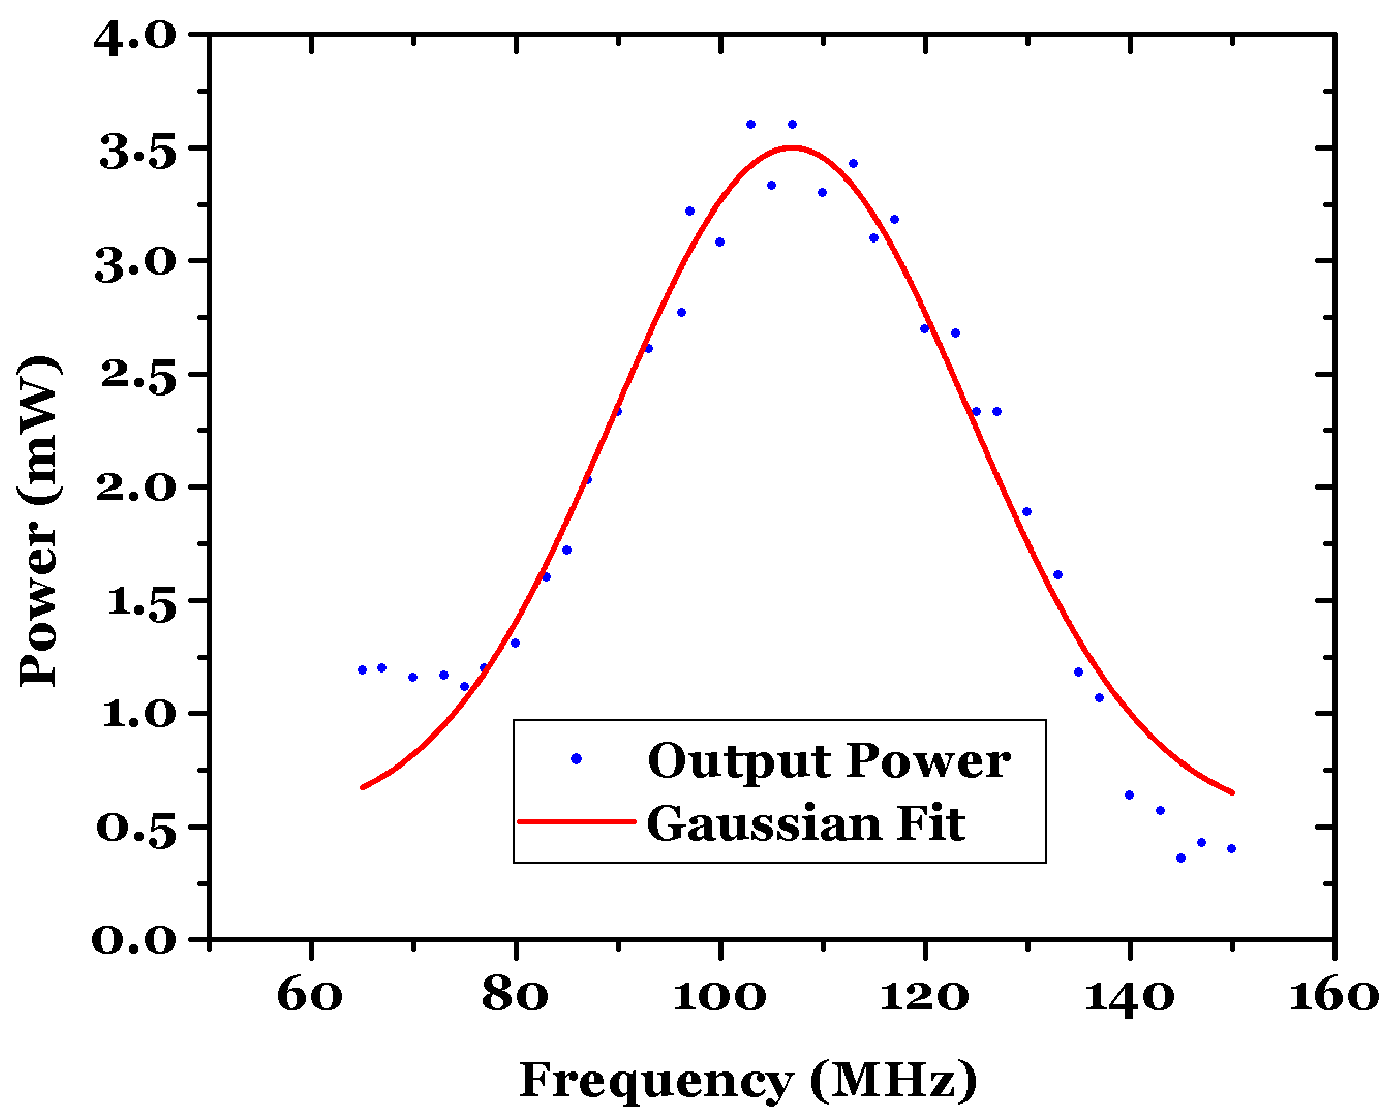
\includegraphics[height=2.5in]{figures/graph.png}

    \caption[Optional: Short caption to appear in List of
    Figures]{Full caption to appear below the Figure}

    \label{figure1}
\end{figure}

% +--------------------------------------------------------------------+
% |To create cross-references to figures, tables and segments
% |of text, LaTeX provides the following commands:
% |   \label{marker}
% |   \ref{marker}
% |   \pageref{marker}
% | where {marker} is a unique identifier.
% |
% | In the line above, we use \label{figure1} to mark a location
% | we wish to refer to later.  LATEX replaces \ref by the number of
% | the chapter, section, subsection, figure, or table after which the
% | corresponding \label command was issued. \pageref prints the page
% | number of the page where the \label command occurred.
% |
% +--------------------------------------------------------------------+

See the file chapter1.tex for examples of the commands used to
insert a figure or table, add a caption, etc.  Here is an example of
a table:

\begin{table}[ht]

% +--------------------------------------------------------------------+
% | We include the command \begin{center} to center the table
% | horizontally on the page.  Note use of the command \end{center}
% | to turn off centering after the table is defined.
% +--------------------------------------------------------------------+
    \begin{center}

% +--------------------------------------------------------------------+
% | The table is created with this command
% |
% | \begin{tabular}[pos]{table spec}
% |
% | The "pos" argument specifies the vertical position of the table
% | relative to the baseline of the surrounding text.  Use t, b, or c
% | to specify alignment at the top, bottom, or center.
% |
% | The "table spec" command defines the format of the table
% |   l for a column of left-aligned text
% |   r for a column of right-aligned text
% |   c for centered text
% |   p{width} for a column containing justified text with line breaks
% |   | for a vertical line
% |
% |  In this example, the caption is made to appear above the table
% |  by positioning the \caption command before the \begin{tabular
% |  command. To position the caption below the table, insert the
% |  \caption command after the \end{tabular} command.
% +--------------------------------------------------------------------+
    \caption{Caption to appear above the table}
    \begin{tabular}[c]{|c|c|c|}
        \hline
        Column 1 Heading & Column 2 Heading & Column 3 Heading \\
        \hline
        Col 1 Row 1 & Col 2 Row 1 & Col 3 Row 1\\
        Col 1 Row 2 & Col 2 Row 2 & Col 3 Row 2\\
        Col 1 Row 3 & Col 2 Row 3 & Col 3 Row 3\\
        \hline
    \end{tabular}

    \label{table1}
   \end{center}
\end{table}



% +--------------------------------------------------------------------+
% | Replace \section headings below with the title of your
% | subsections.  LaTeX will automatically number the subsections 1.1,
% | 1.2, 1.3, etc.
% +--------------------------------------------------------------------+

\section{Making References to Figures or Tables}
\label{makereference1.1}

It is possible to create cross-references and hyperlinks to items or
sections within your paper.  For example, here is a reference to
Fig.~\ref{figure1} mentioned at the beginning of this chapter and a
reference to the Table~\ref{table1}.

\section{Making a Reference to a Chapter Subsection}
\label{makereference1.2}

In this section, we refer back to text mentioned in
Section~\ref{makereference1.1} on page~\pageref{makereference1.1}.

\section{Making a Citation}
\label{makereference1.3}

Here's an example of a citation to a single
work.~\citep{CT:Weiner:1999} It's also possible to make multiple
citations.~\citep{CT:Phillips:1985, ARP:Loy:1974}

This template uses BibTeX to manage and format citations.  BibTeX is
not the only way to create a bibliography within LaTeX, but it's
generally considered to be the best option for long documents like a
thesis or dissertation.~\citep{CT:Gould:1988}  There are a few more
sample citations in this paragraph so you can see examples of how
in-text references are made and how the bibliography is
formatted.~\citep{ARP:Melinger:1991} See the file "BibTeX Guide.pdf"
for information on how to use BibTeX.

% +--------------------------------------------------------------------+
% | Sample Chapter 2
% +--------------------------------------------------------------------+

\cleardoublepage

% +--------------------------------------------------------------------+
% | Replace "This is Chapter 2" below with the title of your chapter.
% | LaTeX will automatically number the chapters.                      
% +--------------------------------------------------------------------+

\chapter{This is Chapter 2}
\label{makereference2}

To refer to Chapter~\ref{makereference1}, use the slash ref command
along with the "makereference" label which was assigned back at the
beginning of Chapter 1.

\section{Page Number References}
\label{makereference2.1} It is possible to refer to a specific page
number, such as page~\pageref{makereference1}.  Add a slash label
command and a unique name for each page to be referenced later in
the text.

\section{Referring to Sections Within Chapter 1}
\label{makereference2.2} It is possible to refer to sections within
a chapter.  Add a slash label command and a unique name with the
section number for each section to be referenced later in the text.
Her is an example of a figure in section~\ref{makereference1.1} and
an example of a table in section~\ref{makereference1.2}.  In
section~\ref{makereference1.3}, we looked at examples of
bibliographic citations.

% +--------------------------------------------------------------------+
% | Sample Chapter 3
% +--------------------------------------------------------------------+

\cleardoublepage

% +--------------------------------------------------------------------+
% | Replace "This is Chapter 3" below with the title of your chapter.
% | LaTeX will automatically number the chapters.                      
% +--------------------------------------------------------------------+

\chapter{This is Chapter 3}
\label{makereference3}

Here are more examples of references to previous sections.  In
Chapter~\ref{makereference1} there were several sections, including
section~\ref{makereference1.1}, section~\ref{makereference1.2}, and
section~\ref{makereference1.3}.

Likewise, in Chapter~\ref{makereference2}, there are
sections~\ref{makereference2.1} and ~\ref{makereference2.2}.


% +--------------------------------------------------------------------+
% | Uncomment the lines below to add additional chapters.
% +--------------------------------------------------------------------+

%\input{chapter4.tex}
%\input{chapter5.tex}

% +--------------------------------------------------------------------+
% | References
% +--------------------------------------------------------------------+

% +--------------------------------------------------------------------+
% | Included for Gather Purpose only.  Do NOT uncomment the next line.
%input "references.bib"
% | In order for the WinEDT editor to index references correctly, it
% | has to know where the "references.bib" file resides.  This
% | command will be ignored completely by LaTeX
% |
% | WinEDT can read file path names with either "\" or "/". LaTeX,
% | however,doesn't like "\", so it's easier to store a path name
% | using forward slashes "/".
% +--------------------------------------------------------------------+

\cleardoublepage
\phantomsection

% +--------------------------------------------------------------------+
% | This template uses the BibTeX program to format references.  The
% | lines below create a separate Bibliography section and add
% | an entry for "Bibliography" to the Table of Contents.  The actual
% | data for your references (author, title, journal, date, etc.) are
% | entered in the references.bib file.  See "Citations and Bibliography"
% | for details on to creating citations and formatting references.
% +--------------------------------------------------------------------+

\addcontentsline{toc}{chapter}{Bibliography}
\bibdata{references}
\bibliography{references}

% +--------------------------------------------------------------------+
% | The following commands add the appendices  To add or delete
% | appendices, add or remove the line
% |
% |     \input{appendixX.tex}
% |
% | where "X" is the letter designation of the appendix (A, B, C,
% | etc.) You should have one \input{appendixX.tex} line and a
% | corresponding file appendixX.tex for each appendix.
% |
% |If you do not have any appendices, comment out or delete the three
% |lines below.
% +--------------------------------------------------------------------+

\appendix
% +--------------------------------------------------------------------+
% | Appendix A Page (Optional)                                         
% +--------------------------------------------------------------------+

\cleardoublepage

\chapter{Title for This Appendix}

\label{Appendix:Key1}

Enter the content for Appendix A in the appendixA.tex file.  If you
do not have an Appendix A, see comments in the etdrtemplate.tex file
for instructions on how to remove this page.

% +--------------------------------------------------------------------+
% | Appendix B Page (Optional)                                         
% +--------------------------------------------------------------------+

\cleardoublepage

\chapter{Title for This Appendix}
\label{Appendix:Key2}

Enter the content for Appendix B in the appendixB.tex file. If you
do not have an Appendix B, see comments in the etdrtemplate.tex file
for instructions on how to remove this page.


\end{document}

% +--------------------------------------------------------------------+
% | Template Revisions
% |
% | 9/14/06: Removed typos
% | 3/29/13: Removed hypernat package
% | 4/5/13: Changed to plain bib style
% | 5/17/13: added /cleardoublepage and /phantomsection to
% |          /bibliography to correct TOC page problem
% | 5/17/13: Fixed TOC problem with Dedication, Preface, etc.
% | 12/16/15: Added tocloft package to produce leader dots for all
% |           entries in the table of contents.
% |           Added geometry package to specify 1 inch margins.
% |           Removed unnecessary color specifications.
% |           Changed to \citep for citations.
% | 2/9/2016: Replaced \bibpunct with \setcitestyle.
% |           Changed to unsrtnat style
% |           Added natbib.pdf and Citations and Bibliography.pdf files
% |
% +--------------------------------------------------------------------+
